% Options for packages loaded elsewhere
\PassOptionsToPackage{unicode}{hyperref}
\PassOptionsToPackage{hyphens}{url}
%
\documentclass[
  14pt,
  letterpaper,
  ignorenonframetext,
  aspectratio=169,
  handout]{beamer}
\usepackage{pgfpages}
\setbeamertemplate{caption}[numbered]
\setbeamertemplate{caption label separator}{: }
\setbeamercolor{caption name}{fg=normal text.fg}
\beamertemplatenavigationsymbolsempty
% Prevent slide breaks in the middle of a paragraph
\widowpenalties 1 10000
\raggedbottom
\setbeamertemplate{part page}{
  \centering
  \begin{beamercolorbox}[sep=16pt,center]{part title}
    \usebeamerfont{part title}\insertpart\par
  \end{beamercolorbox}
}
\setbeamertemplate{section page}{
  \centering
  \begin{beamercolorbox}[sep=12pt,center]{part title}
    \usebeamerfont{section title}\insertsection\par
  \end{beamercolorbox}
}
\setbeamertemplate{subsection page}{
  \centering
  \begin{beamercolorbox}[sep=8pt,center]{part title}
    \usebeamerfont{subsection title}\insertsubsection\par
  \end{beamercolorbox}
}
\AtBeginPart{
  \frame{\partpage}
}
\AtBeginSection{
  \ifbibliography
  \else
    \frame{\sectionpage}
  \fi
}
\AtBeginSubsection{
  \frame{\subsectionpage}
}

\usepackage{amsmath,amssymb}
\usepackage{lmodern}
\usepackage{iftex}
\ifPDFTeX
  \usepackage[T1]{fontenc}
  \usepackage[utf8]{inputenc}
  \usepackage{textcomp} % provide euro and other symbols
\else % if luatex or xetex
  \usepackage{unicode-math}
  \defaultfontfeatures{Scale=MatchLowercase}
  \defaultfontfeatures[\rmfamily]{Ligatures=TeX,Scale=1}
  \setmainfont[Scale=MatchLowercase]{SF Pro Text Light}
  \setmathfont[]{STIX Two Math}
\fi
\usetheme[]{boxes}
\usecolortheme{wolverine}
\usefonttheme{serif} % use mainfont rather than sansfont for slide text
% Use upquote if available, for straight quotes in verbatim environments
\IfFileExists{upquote.sty}{\usepackage{upquote}}{}
\IfFileExists{microtype.sty}{% use microtype if available
  \usepackage[]{microtype}
  \UseMicrotypeSet[protrusion]{basicmath} % disable protrusion for tt fonts
}{}
\makeatletter
\@ifundefined{KOMAClassName}{% if non-KOMA class
  \IfFileExists{parskip.sty}{%
    \usepackage{parskip}
  }{% else
    \setlength{\parindent}{0pt}
    \setlength{\parskip}{6pt plus 2pt minus 1pt}}
}{% if KOMA class
  \KOMAoptions{parskip=half}}
\makeatother
\usepackage{xcolor}
\newif\ifbibliography
\setlength{\emergencystretch}{3em} % prevent overfull lines
\setcounter{secnumdepth}{-\maxdimen} % remove section numbering


\providecommand{\tightlist}{%
  \setlength{\itemsep}{0pt}\setlength{\parskip}{0pt}}\usepackage{longtable,booktabs,array}
\usepackage{calc} % for calculating minipage widths
\usepackage{caption}
% Make caption package work with longtable
\makeatletter
\def\fnum@table{\tablename~\thetable}
\makeatother
\usepackage{graphicx}
\makeatletter
\def\maxwidth{\ifdim\Gin@nat@width>\linewidth\linewidth\else\Gin@nat@width\fi}
\def\maxheight{\ifdim\Gin@nat@height>\textheight\textheight\else\Gin@nat@height\fi}
\makeatother
% Scale images if necessary, so that they will not overflow the page
% margins by default, and it is still possible to overwrite the defaults
% using explicit options in \includegraphics[width, height, ...]{}
\setkeys{Gin}{width=\maxwidth,height=\maxheight,keepaspectratio}
% Set default figure placement to htbp
\makeatletter
\def\fps@figure{htbp}
\makeatother

\captionsetup[figure]{labelformat=empty}
\usepackage{pgfpages}
\setbeamertemplate{itemize item}[circle]
\setbeamertemplate{footline}[frame number]{}
\mode<handout>{\pgfpagesuselayout{6 on 1}[letterpaper, border shrink=8mm]}
\AtBeginSection{%
   \begin{frame}
       \tableofcontents[currentsection]
   \end{frame}
}
\usepackage{tikz}
\usetikzlibrary{positioning,arrows,calc}
\tikzset{
  modal/.style={>=stealth',
    shorten >=1pt,
    shorten <=1pt,
    auto,
   node distance=1.5cm,
   label distance=2pt,
   semithick},
 every label/.style={phantom,align=left},
 world/.style = {circle,draw,minimum size=0.5cm,fill=gray!15},
 modal every node/.style={world},
 point/.style={circle,draw,inner sep=0.5mm,fill=black},
 phantom/.style={rectangle,inner sep=0pt,draw=none,fill=none},
 reflexive above/.style={->,loop,looseness=7,in=60,out=120},
 reflexive below/.style={->,loop,looseness=7,in=240,out=300},
 reflexive left/.style={->,loop,looseness=7,in=150,out=210},
 reflexive right/.style={->,loop,looseness=7,in=30,out=330}}
\makeatletter
\makeatother
\makeatletter
\makeatother
\makeatletter
\@ifpackageloaded{caption}{}{\usepackage{caption}}
\AtBeginDocument{%
\ifdefined\contentsname
  \renewcommand*\contentsname{Table of contents}
\else
  \newcommand\contentsname{Table of contents}
\fi
\ifdefined\listfigurename
  \renewcommand*\listfigurename{List of Figures}
\else
  \newcommand\listfigurename{List of Figures}
\fi
\ifdefined\listtablename
  \renewcommand*\listtablename{List of Tables}
\else
  \newcommand\listtablename{List of Tables}
\fi
\ifdefined\figurename
  \renewcommand*\figurename{Figure}
\else
  \newcommand\figurename{Figure}
\fi
\ifdefined\tablename
  \renewcommand*\tablename{Table}
\else
  \newcommand\tablename{Table}
\fi
}
\@ifpackageloaded{float}{}{\usepackage{float}}
\floatstyle{ruled}
\@ifundefined{c@chapter}{\newfloat{codelisting}{h}{lop}}{\newfloat{codelisting}{h}{lop}[chapter]}
\floatname{codelisting}{Listing}
\newcommand*\listoflistings{\listof{codelisting}{List of Listings}}
\makeatother
\makeatletter
\@ifpackageloaded{caption}{}{\usepackage{caption}}
\@ifpackageloaded{subcaption}{}{\usepackage{subcaption}}
\makeatother
\makeatletter
\@ifpackageloaded{tcolorbox}{}{\usepackage[many]{tcolorbox}}
\makeatother
\makeatletter
\@ifundefined{shadecolor}{\definecolor{shadecolor}{rgb}{.97, .97, .97}}
\makeatother
\makeatletter
\makeatother
\ifLuaTeX
  \usepackage{selnolig}  % disable illegal ligatures
\fi
\IfFileExists{bookmark.sty}{\usepackage{bookmark}}{\usepackage{hyperref}}
\IfFileExists{xurl.sty}{\usepackage{xurl}}{} % add URL line breaks if available
\urlstyle{same} % disable monospaced font for URLs
\hypersetup{
  pdftitle={Honors Logic, Lecture 12 - Modal Logic},
  pdfauthor={Brian Weatherson},
  hidelinks,
  pdfcreator={LaTeX via pandoc}}

\title{Honors Logic, Lecture 12 - Modal Logic}
\author{Brian Weatherson}
\date{2022-10-10}

\begin{document}
\frame{\titlepage}
\ifdefined\Shaded\renewenvironment{Shaded}{\begin{tcolorbox}[boxrule=0pt, interior hidden, sharp corners, enhanced, breakable, borderline west={3pt}{0pt}{shadecolor}, frame hidden]}{\end{tcolorbox}}\fi

\begin{frame}{Access}
\protect\hypertarget{access}{}
We can think, a little picturesquely, as the accessibility relation
being a `step' between worlds.

\begin{itemize}[<+->]
\tightlist
\item
  If \(wRy\), then you can `step' from \(w\) to \(y\).
\item
  \(\Box A\) means that anywhere you can step to from \(w\) is a world
  where \(A\) is true.
\item
  And \(\Box \Box A\) means that anywhere you can get to in two steps
  from \(w\) is a world where \(A\) is true.
\end{itemize}
\end{frame}

\begin{frame}{Iterated Modalities}
\protect\hypertarget{iterated-modalities}{}
We can run the rules in sequence.

\begin{itemize}[<+->]
\tightlist
\item
  What does it take for \(\Diamond \Diamond A\) to be true at \(w\)?
\item
  It is for \(\Diamond A\) to be true at some \(y\) such that \(wRy\).
\item
  And that means that \(A\) has to be true at some world \(z\) such that
  \(yRz\) (for some \(y\) such that \(wRy)\).
\item
  In the picturesque terms, you can get from \(w\) to an \(A\)-world in
  two steps.
\end{itemize}
\end{frame}

\begin{frame}{Mixed Modalities}
\protect\hypertarget{mixed-modalities}{}
What does it mean for \(\Diamond \Box A\) to be true at \(w\)?

\begin{itemize}[<+->]
\tightlist
\item
  There is some accessible world where \(\Box A\) is true.
\item
  That is, there is some accessible world such that everywhere you can
  go from there, \(A\) is true.
\end{itemize}
\end{frame}

\begin{frame}{Mixed Modalities}
\protect\hypertarget{mixed-modalities-1}{}
What does it mean for \(\Box \Diamond A\) to be true at \(w\)?

\begin{itemize}[<+->]
\tightlist
\item
  At all accessible worlds, \(\Diamond A\) is true.
\item
  That is, wherever you go, you can get to there is some accessible
  world such that everywhere you can go from there, \(A\) is true.
\end{itemize}
\end{frame}

\begin{frame}{Longer Sentences}
\protect\hypertarget{longer-sentences}{}
What does it mean for \(\Box(p \vee (q \supset \Diamond r))\) to be true
at \(w\)?

\begin{itemize}[<+->]
\tightlist
\item
  It's for \(p \vee (q \supset \Diamond r)\) to be true everywhere you
  can get to (in one step) from \(w\).
\item
  That is, at every one of those worlds, either \(p\) is true or
  \(q \supset \Diamond r\) is true.
\item
  That is, at every one of those worlds, either \(p\) is true, or \(q\)
  is false, or \(\Diamond r\) is true.
\item
  That is, at every one of those worlds, either \(p\) is true, or \(q\)
  is false, or there is some world you can get to where \(r\) is true.
\end{itemize}
\end{frame}

\begin{frame}{Box and connectives}
\protect\hypertarget{box-and-connectives}{}
The general rule is just to apply the rules for sentences inside the
brackets at each world in \(W\), and then apply the rule for \(\Box\) or
\(\Diamond\). But there are three special cases worth thinking about.

\begin{itemize}[<+->]
\tightlist
\item
  \(\Box(A \wedge B)\) means that all accessible worlds are \(A\) and
  \(B\) worlds.
\item
  \(\Box(A \vee B)\) means that all accessible worlds make at least one
  of \(A\) and \(B\) true.
\item
  \(\Box(A \supset B)\) means that all accessible \(A\)-worlds are
  \(B\)-worlds.
\end{itemize}

We'll use that last one a lot.
\end{frame}

\begin{frame}{A Weird Special Case}
\protect\hypertarget{a-weird-special-case}{}
If for some \(w\) there is no \(x\) such that \(wRx\), then at \(w\):

\begin{enumerate}[<+->]
\tightlist
\item
  Every box sentence is true.
\item
  Every diamond sentence is false.
\end{enumerate}

\begin{itemize}[<+->]
\tightlist
\item
  This is weird; normally box something is a much \textbf{stronger}
  claim than diamond, but this is a weird exception.
\end{itemize}
\end{frame}

\begin{frame}{A Weird Special Case}
\protect\hypertarget{a-weird-special-case-1}{}
I normally wouldn't mention this, because it's not something that's of
particular philosophical significance.

\begin{itemize}[<+->]
\tightlist
\item
  Except, when we're doing trees/tableau, we start out with no R
  relations at all, so we end up in this special case a lot. It's
  somewhat annoying to spend so much time doing something with no
  philosophical relevance, but it is mathematicaly convenient to have
  these cases around.
\end{itemize}
\end{frame}

\begin{frame}
I'm going to go through this table and show how each of them can be
false.

\begin{enumerate}[<+->]
\tightlist
\item
  \(\Box(A \vee B) \supset (\Box A \vee \Box B)\)
\item
  \((\Diamond A \wedge \Diamond B) \supset \Diamond (A \wedge B)\)
\item
  \(A \supset \Box A\)
\item
  \(\Box A \supset A\)
\item
  \(\Box \Diamond A \supset B\)
\item
  \(\Box \Diamond A \supset A\)
\item
  \(\Box \Box A \supset \Box A\)
\item
  \(\Box A \supset \Box \Box A\)
\item
  \(\Box \Diamond A \supset \Diamond \Box A\)
\item
  \(\Box A \supset \Diamond A\)
\end{enumerate}
\end{frame}

\begin{frame}{\(\Box(A \vee B) \supset (\Box A \vee \Box B)\)}
\protect\hypertarget{boxa-vee-b-supset-box-a-vee-box-b}{}
\begin{columns}
    \begin{column}{0.65\textwidth}
        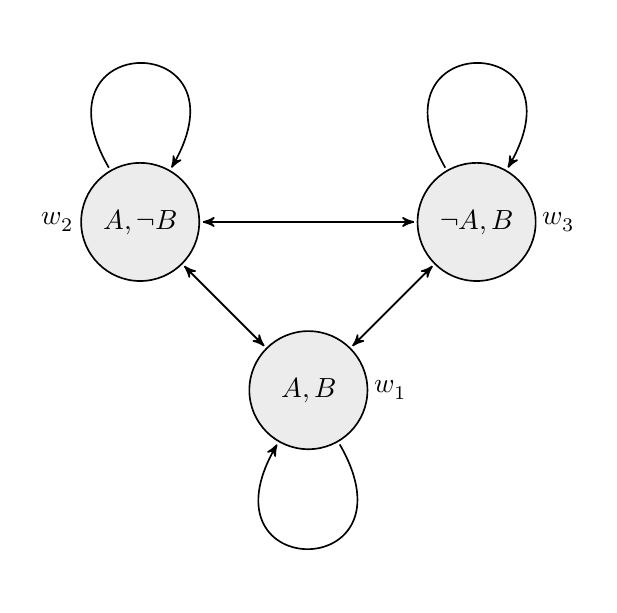
\begin{tikzpicture}[scale=0.6,modal,world/.append style={minimum size=1.5cm}]
      \node[world] (w1) [label=right:$w_1$]{$A,B$}; 
      \node[world] (w2) [label=left:$w_2$, above left=of w1]{$A, \neg B$}; 
      \node[world] (w3) [label=right:$w_3$, above right=of w1] {$\neg A, B$};
      \draw[->] (w1) to (w2);
      \draw[->] (w1) to (w3);
      \draw[->] (w2) to (w1);
      \draw[->] (w3) to (w1);
      \draw[->] (w3) to (w2);
      \draw[->] (w2) to (w3);
      \path[->] (w2) edge[reflexive above] (w2);
      \path[->] (w3) edge[reflexive above] (w3);
      \path[->] (w1) edge[reflexive below] (w1);
    \end{tikzpicture}
    \end{column}
    \begin{column}{0.3\textwidth}
At all points, either $A$ or $B$ is true, so $\Box(A \vee B)$ is true.  

\bigskip

But $\Box A$ and $\Box B$ are false everywhere.  So the conditional is false everywhere.
\end{column}
\end{columns}
\end{frame}

\begin{frame}{\(\Box(A \vee B) \supset (\Box A \vee \Box B)\)}
\protect\hypertarget{boxa-vee-b-supset-box-a-vee-box-b-1}{}
\begin{columns}
    \begin{column}{0.65\textwidth}
        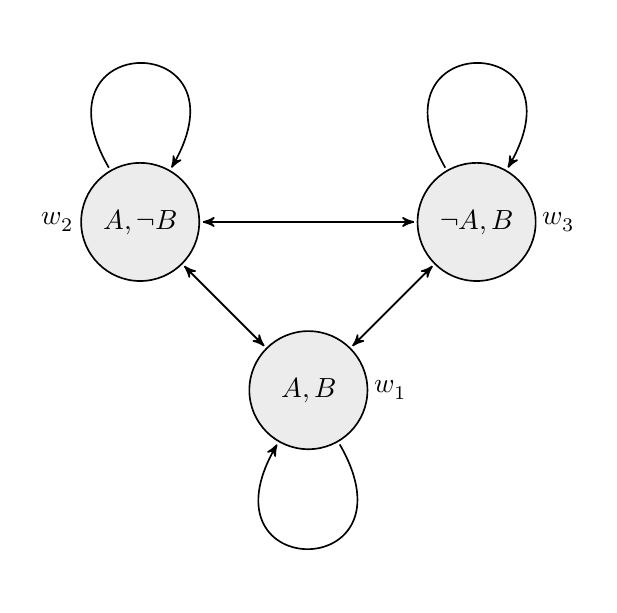
\begin{tikzpicture}[scale=0.6,modal,world/.append style={minimum size=1.5cm}]
      \node[world] (w1) [label=right:$w_1$]{$A,B$}; 
      \node[world] (w2) [label=left:$w_2$, above left=of w1]{$A, \neg B$}; 
      \node[world] (w3) [label=right:$w_3$, above right=of w1] {$\neg A, B$};
      \draw[->] (w1) to (w2);
      \draw[->] (w1) to (w3);
      \draw[->] (w2) to (w1);
      \draw[->] (w3) to (w1);
      \draw[->] (w3) to (w2);
      \draw[->] (w2) to (w3);
      \path[->] (w2) edge[reflexive above] (w2);
      \path[->] (w3) edge[reflexive above] (w3);
      \path[->] (w1) edge[reflexive below] (w1);
    \end{tikzpicture}
    \end{column}
    \begin{column}{0.3\textwidth}
Note that this is overkill. We just need to show that the formula can be false somewhere in order to show that it is not a theorem.
\end{column}
\end{columns}
\end{frame}

\begin{frame}{\((\Diamond A \wedge \Diamond B) \supset \Diamond (A \wedge B)\)}
\protect\hypertarget{diamond-a-wedge-diamond-b-supset-diamond-a-wedge-b}{}
\begin{columns}
    \begin{column}{0.65\textwidth}
        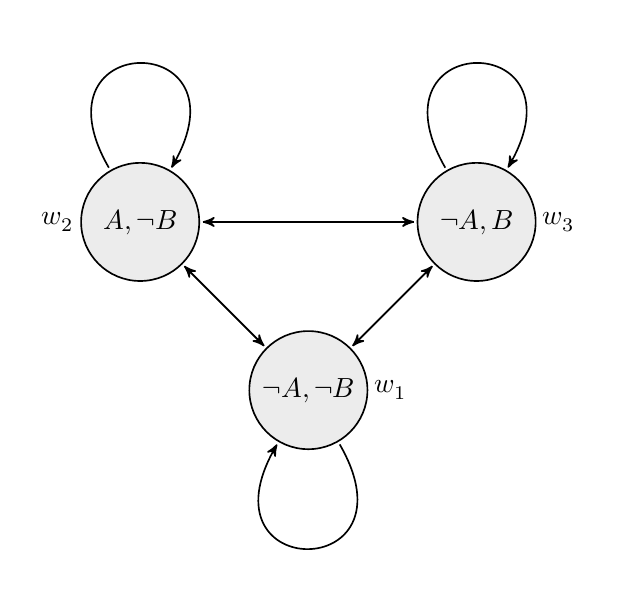
\begin{tikzpicture}[scale=0.5,modal,world/.append style={minimum size=1.5cm}]
      \node[world] (w1) [label=right:$w_1$]{$\neg A, \neg B$}; 
      \node[world] (w2) [label=left:$w_2$, above left=of w1]{$A, \neg B$}; 
      \node[world] (w3) [label=right:$w_3$, above right=of w1] {$\neg A, B$};
      \draw[->] (w1) to (w2);
      \draw[->] (w1) to (w3);
      \draw[->] (w2) to (w1);
      \draw[->] (w3) to (w1);
      \draw[->] (w3) to (w2);
      \draw[->] (w2) to (w3);
      \path[->] (w2) edge[reflexive above] (w2);
      \path[->] (w3) edge[reflexive above] (w3);
      \path[->] (w1) edge[reflexive below] (w1);
    \end{tikzpicture}
    \end{column}
    \begin{column}{0.33\textwidth}

At $w_1$, we have $\Diamond A \wedge \Diamond B$ true. 

 \bigskip

But nowhere is $A \wedge B$ true, so $\Diamond(A \wedge B)$ is false at $w_1$. So the conditional is false. 

 \bigskip

Again, this is overkill.
\end{column}
\end{columns}
\end{frame}

\begin{frame}{\(A \supset \Box A\)}
\protect\hypertarget{a-supset-box-a}{}
\begin{columns}
    \begin{column}{0.45\textwidth}
        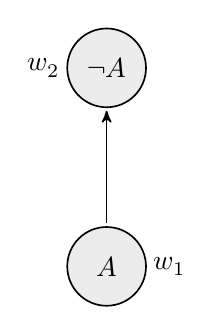
\begin{tikzpicture}[scale=0.6,modal,world/.append style={minimum size=1cm}]
      \node[world] (w1) [label=right:$w_1$]{$A$}; 
      \node[world] (w2) [label=left:$w_2$, above =of w1]{$\neg A$}; 
      \draw[->] (w1) to (w2);
    \end{tikzpicture}
    \end{column}
    \begin{column}{0.5\textwidth}
    \begin{itemize}
    \item At $w_1$ $A$ is true.
    \item But $\Box A$ is false, since $w_1$ can access $w_2$, and $A$ is false there.
    \item So $A \supset \Box A$ is false.
    \end{itemize}
  \end{column}
\end{columns}
\end{frame}

\begin{frame}{\(\Box A \supset A\)}
\protect\hypertarget{box-a-supset-a}{}
\begin{columns}
    \begin{column}{0.45\textwidth}
        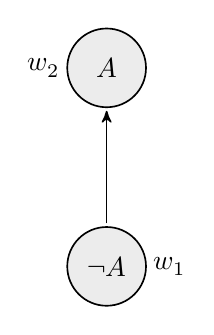
\begin{tikzpicture}[scale=0.6,modal,world/.append style={minimum size=1cm}]
      \node[world] (w1) [label=right:$w_1$]{$\neg A$}; 
      \node[world] (w2) [label=left:$w_2$, above =of w1]{$A$}; 
      \draw[->] (w1) to (w2);
    \end{tikzpicture}
    \end{column}
    \begin{column}{0.5\textwidth}
    \begin{itemize}
    \item At $w_1$ $\Box A$ is true. The only accessible world is $w_2$, and $A$ is true there.
    \item But $A$ is false there.
    \item So $\Box A \supset A$ is false.
    \end{itemize}
  \end{column}
\end{columns}
\end{frame}

\begin{frame}{\(\Box \Diamond A \supset B\)}
\protect\hypertarget{box-diamond-a-supset-b}{}
\begin{columns}
    \begin{column}{0.45\textwidth}
        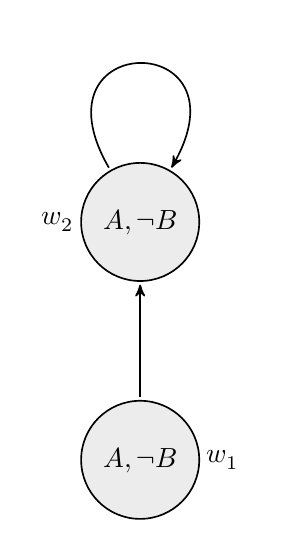
\begin{tikzpicture}[scale=0.6,modal,world/.append style={minimum size=1.5cm}]
      \node[world] (w1) [label=right:$w_1$]{$A, \neg B$}; 
      \node[world] (w2) [label=left:$w_2$, above =of w1]{$A, \neg B$}; 
      \draw[->] (w1) to (w2);
     \path[->] (w2) edge[reflexive above] (w2);
    \end{tikzpicture}
    \end{column}
    \begin{column}{0.5\textwidth}
    \begin{itemize}
    \item At $w_1$ $\Box \Diamond A$ is true. The only accessible world is $w_2$, and $\Diamond A$ is true there. (Why?)
    \item But $B$ is false at $w_1$.
    \item So $\Box \Diamond A \supset B$ is false.
    \end{itemize}
  \end{column}
\end{columns}
\end{frame}

\begin{frame}{\(\Box \Diamond A \supset A\)}
\protect\hypertarget{box-diamond-a-supset-a}{}
\begin{columns}
    \begin{column}{0.45\textwidth}
        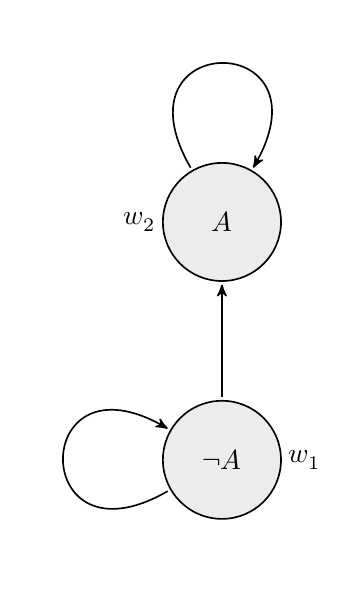
\begin{tikzpicture}[scale=0.6,modal,world/.append style={minimum size=1.5cm}]
      \node[world] (w1) [label=right:$w_1$]{$\neg A$}; 
      \node[world] (w2) [label=left:$w_2$, above =of w1]{$A$}; 
      \draw[->] (w1) to (w2);
     \path[->] (w2) edge[reflexive above] (w2);
     \path[->] (w1) edge[reflexive left] (w1);
    \end{tikzpicture}
    \end{column}
    \begin{column}{0.5\textwidth}
    \begin{itemize}
    \item At $w_1$ $\Box \Diamond A$ is true. At every world, $w_2$ is accessible, and $A$ is true there.
    \item But $A$ is false at $w_1$.
    \item So $\Box \Diamond A \supset A$ is false at $w_1$.
    \end{itemize}
  \end{column}
\end{columns}
\end{frame}

\begin{frame}{\(\Box \Box A \supset \Box A\)}
\protect\hypertarget{box-box-a-supset-box-a}{}
\begin{columns}
    \begin{column}{0.45\textwidth}
        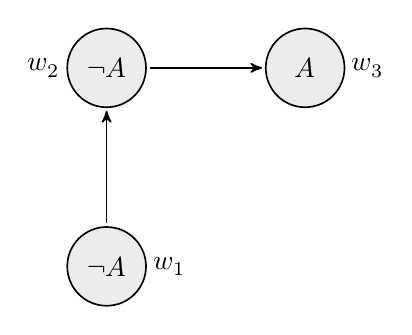
\begin{tikzpicture}[scale=0.5,modal,world/.append style={minimum size=1cm}]
      \node[world] (w1) [label=right:$w_1$]{$\neg A$}; 
      \node[world] (w2) [label=left:$w_2$, above =of w1]{$\neg A$}; 
      \node[world] (w3) [label=right:$w_3$, right =of w2]{$A$}; 
      \draw[->] (w1) to (w2);
      \draw[->] (w2) to (w3);
%     \path[->] (w2) edge[reflexive above] (w2);
%     \path[->] (w1) edge[reflexive left] (w1);
    \end{tikzpicture}
    \end{column}
    \begin{column}{0.5\textwidth}
    \begin{itemize}
    \item The only world $w_2$ can access is $w_3$, and $A$ is true there, so $\Box A$ is true at $w_2$.
    \item The only world $w_1$ can access is $w_2$, and $\Box A$ is true there, so $\Box \Box A$ is true at $w_1$.
    \item But $\Box A$ is false at $w_1$.
    \item So $\Box \Box A \supset \Box A$ is false at $w_1$.
    \end{itemize}
  \end{column}
\end{columns}
\end{frame}

\begin{frame}{\(\Box A \supset \Box \Box A\)}
\protect\hypertarget{box-a-supset-box-box-a}{}
\begin{columns}
    \begin{column}{0.45\textwidth}
        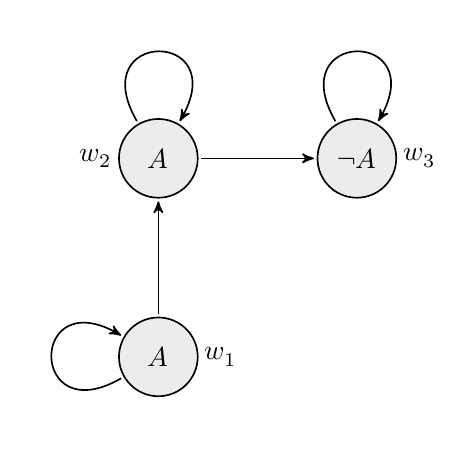
\begin{tikzpicture}[scale=0.5,modal,world/.append style={minimum size=1cm}]
      \node[world] (w1) [label=right:$w_1$]{$A$}; 
      \node[world] (w2) [label=left:$w_2$, above =of w1]{$A$}; 
      \node[world] (w3) [label=right:$w_3$, right =of w2]{$\neg A$}; 
      \draw[->] (w1) to (w2);
      \draw[->] (w2) to (w3);
     \path[->] (w2) edge[reflexive above] (w2);
     \path[->] (w3) edge[reflexive above] (w3);
     \path[->] (w1) edge[reflexive left] (w1);
    \end{tikzpicture}
    \end{column}
    \begin{column}{0.5\textwidth}
    \begin{itemize}
    \item Since $A$ is false at $w_3$, and $w_2$ can access $w_3$, $\Box A$ is false at $w_2$.
    \item Since $\Box A$ is false at $w_2$, and $w_1$ can access $w_2$, $\Box \Box A$ is false at $w_1$.
    \item But $\Box A$ is true at $w_1$.
    \item So $\Box A \supset \Box \Box A$ is false at $w_1$.
    \end{itemize}
       \end{column}
\end{columns}
\end{frame}

\begin{frame}{\(\Box A \supset \Diamond A\)}
\protect\hypertarget{box-a-supset-diamond-a}{}
\begin{columns}
    \begin{column}{0.45\textwidth}
        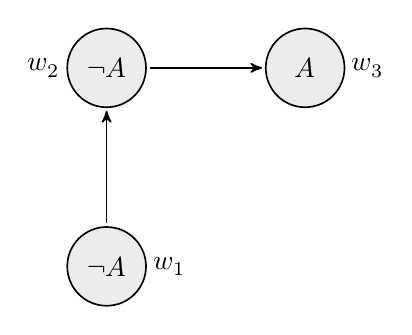
\begin{tikzpicture}[scale=0.5,modal,world/.append style={minimum size=1cm}]
      \node[world] (w1) [label=right:$w_1$]{$\neg A$}; 
      \node[world] (w2) [label=left:$w_2$, above =of w1]{$\neg A$}; 
      \node[world] (w3) [label=right:$w_3$, right =of w2]{$A$}; 
      \draw[->] (w1) to (w2);
      \draw[->] (w2) to (w3);
%     \path[->] (w2) edge[reflexive above] (w2);
%     \path[->] (w1) edge[reflexive left] (w1);
    \end{tikzpicture}
    \end{column}
    \begin{column}{0.5\textwidth}
    \begin{itemize}
    \item Focus on $w_3$.
    \item There is no accessible world where $A$ is false, so $\Box A$ is true there.
    \item But there is no accessible world where $A$ is true, so $\Diamond A$ is false there.
    \item So $\Box A \supset \Diamond A$ is false there.
    \end{itemize}
\end{column}
\end{columns}
\end{frame}

\begin{frame}{\(\Box A \supset \Diamond A\)}
\protect\hypertarget{box-a-supset-diamond-a-1}{}
\begin{columns}
    \begin{column}{0.45\textwidth}
        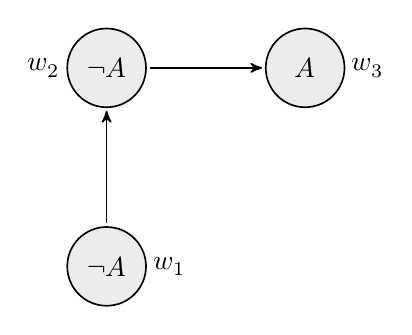
\begin{tikzpicture}[scale=0.5,modal,world/.append style={minimum size=1cm}]
      \node[world] (w1) [label=right:$w_1$]{$\neg A$}; 
      \node[world] (w2) [label=left:$w_2$, above =of w1]{$\neg A$}; 
      \node[world] (w3) [label=right:$w_3$, right =of w2]{$A$}; 
      \draw[->] (w1) to (w2);
      \draw[->] (w2) to (w3);
%     \path[->] (w2) edge[reflexive above] (w2);
%     \path[->] (w1) edge[reflexive left] (w1);
    \end{tikzpicture}
    \end{column}
    \begin{column}{0.5\textwidth}
    Whenever there are no accessible worlds, the following two weird things happen.
    \begin{enumerate}
    \item All $\Box$-sentences (i.e., sentences that start with a $\Box$ that takes scope over the whole sentence) are true.
    \item All $\Diamond$-sentences (i.e., sentences that start with a $\Diamond$ that takes scope over the whole sentence) are false.
    \end{enumerate}
   \end{column}
\end{columns}
\end{frame}



\end{document}
